\documentclass[10pt]{beamer}
\usefonttheme{professionalfonts,serif}
\def\newblock{\hskip .11em plus .33em minus .07em}
\usepackage[numbers,sort]{natbib}
\renewcommand{\rmdefault}{psbx}
\usepackage[utf8]{inputenc}
\usepackage[T1]{fontenc}
\usepackage{textcomp}
\usepackage{eulervm}

\usetheme{default}           % tips from David Blei
\useinnertheme{circles}
\useoutertheme{infolines}
\setbeamertemplate{headline}{}
\setbeamertemplate{navigation symbols}{}
\setbeamerfont{itemize/enumerate subbody}{size=\normalsize}
\setbeamerfont{itemize/enumerate subsubbody}{size=\normalsize}
\usecolortheme{seahorse}
\setbeamersize{text margin left=2mm,text margin right=2mm}

\graphicspath{{../../figures/}}

\definecolor{mypine}{rgb}{0.05,0.45,0.05}
\definecolor{mycyan}{rgb}{0.0,0.9,0.9}
\newcommand{\Red}{\textcolor{red}}
\newcommand{\Blue}{\textcolor{blue}}
\newcommand{\Green}{\textcolor{mypine}}
\newcommand{\PineGreen}{\textcolor{mypine}}
\newcommand{\Magenta}{\textcolor{magenta}}
\newcommand{\Cyan}{\textcolor{mycyan}}

\newcommand{\N}{\mathcal{N}}
\newcommand{\R}{\mathbb{R}}
\newcommand{\T}{{\scriptsize^{\top}}}
\newcommand{\D}{\mathcal{D}}
\newcommand{\F}{\mathcal{F}}
\newcommand{\E}{\mathbb{E}}
\newcommand{\V}{\mathbb{V}}
\newcommand{\M}{\mathcal{M}}
\newcommand{\KL}{\mathcal{KL}}
\newcommand{\cut}[1]{}
\newcommand{\trace}{\operatorname{trace}}

\newcommand{\bmu}{{\boldsymbol{\mu}}}
\newcommand{\btheta}{\boldsymbol{\theta}}
\newcommand{\bepsilon}{\boldsymbol{\epsilon}}
\newcommand{\balpha}{\boldsymbol{\alpha}}
\newcommand{\bbeta}{\boldsymbol{\beta}}
\newcommand{\bphi}{\boldsymbol{\phi}}
\newcommand{\bPhi}{\boldsymbol{\Phi}}
\newcommand{\bSigma}{\boldsymbol{\Sigma}}
\newcommand{\bpi}{\boldsymbol{\pi}}
\newcommand{\blambda}{\boldsymbol{\lambda}}

\newcommand{\argmax}{\operatorname{argmax}}
\newcommand{\argmin}{\operatorname{argmin}}
\newcommand{\ci}{{\bot\negthickspace\negthickspace\bot}} % conditional indep.
\newcommand{\neigh}{\operatorname{ne}}
\newcommand{\vectr}[2]{  \left[ \!\!\begin{array}{c} #1 \\
      #2 \end{array} \!\!\right]}
\newcommand{\deff}{\stackrel{\mathrm{def}}{=}}
\newcommand{\deldel}[2]{\frac{\partial #1}{\partial #2}}

\newcommand{\maketilde}{\raisebox{0.4ex}{\tiny $\sim$}}
\newcommand{\bfa}{\mathbf a}
\newcommand{\bfb}{\mathbf b}
\newcommand{\bfe}{\mathbf e}
\newcommand{\bff}{\mathbf f}
\newcommand{\bfk}{\mathbf k}
\newcommand{\bfm}{\mathbf m}
\newcommand{\bfn}{\mathbf n}
\newcommand{\bfp}{\mathbf{p}}
\newcommand{\bfs}{\mathbf s}
\newcommand{\bfu}{\mathbf u}
\newcommand{\bfx}{\mathbf x}
\newcommand{\bfy}{\mathbf y}
\newcommand{\bft}{\mathbf t}
\newcommand{\bfv}{\mathbf v}
\newcommand{\bfw}{\mathbf w}
\newcommand{\bfA}{\mathbf A}
\newcommand{\bfI}{\mathbf I}
\newcommand{\bfK}{\mathbf K}


\title{Moment matching approximation}
\author{Carl Edward Rasmussen}
\date{October 28th, 2016}

\begin{document}


\begin{frame}
\titlepage
\end{frame}


\begin{frame}
\frametitle{Key concepts}

\begin{itemize}
\item in practise, we can (more or less) only compute with Gaussians
\item but the game outcomes are binary
\item how can we approximate a binary variable with a Gaussian?
\item key idea: \Blue{moment matching} approximates the \Blue{effect} of
the binary variable
\end{itemize}

\end{frame}

\begin{frame}
\frametitle{Approximating a step by a Gaussian?}

\centerline{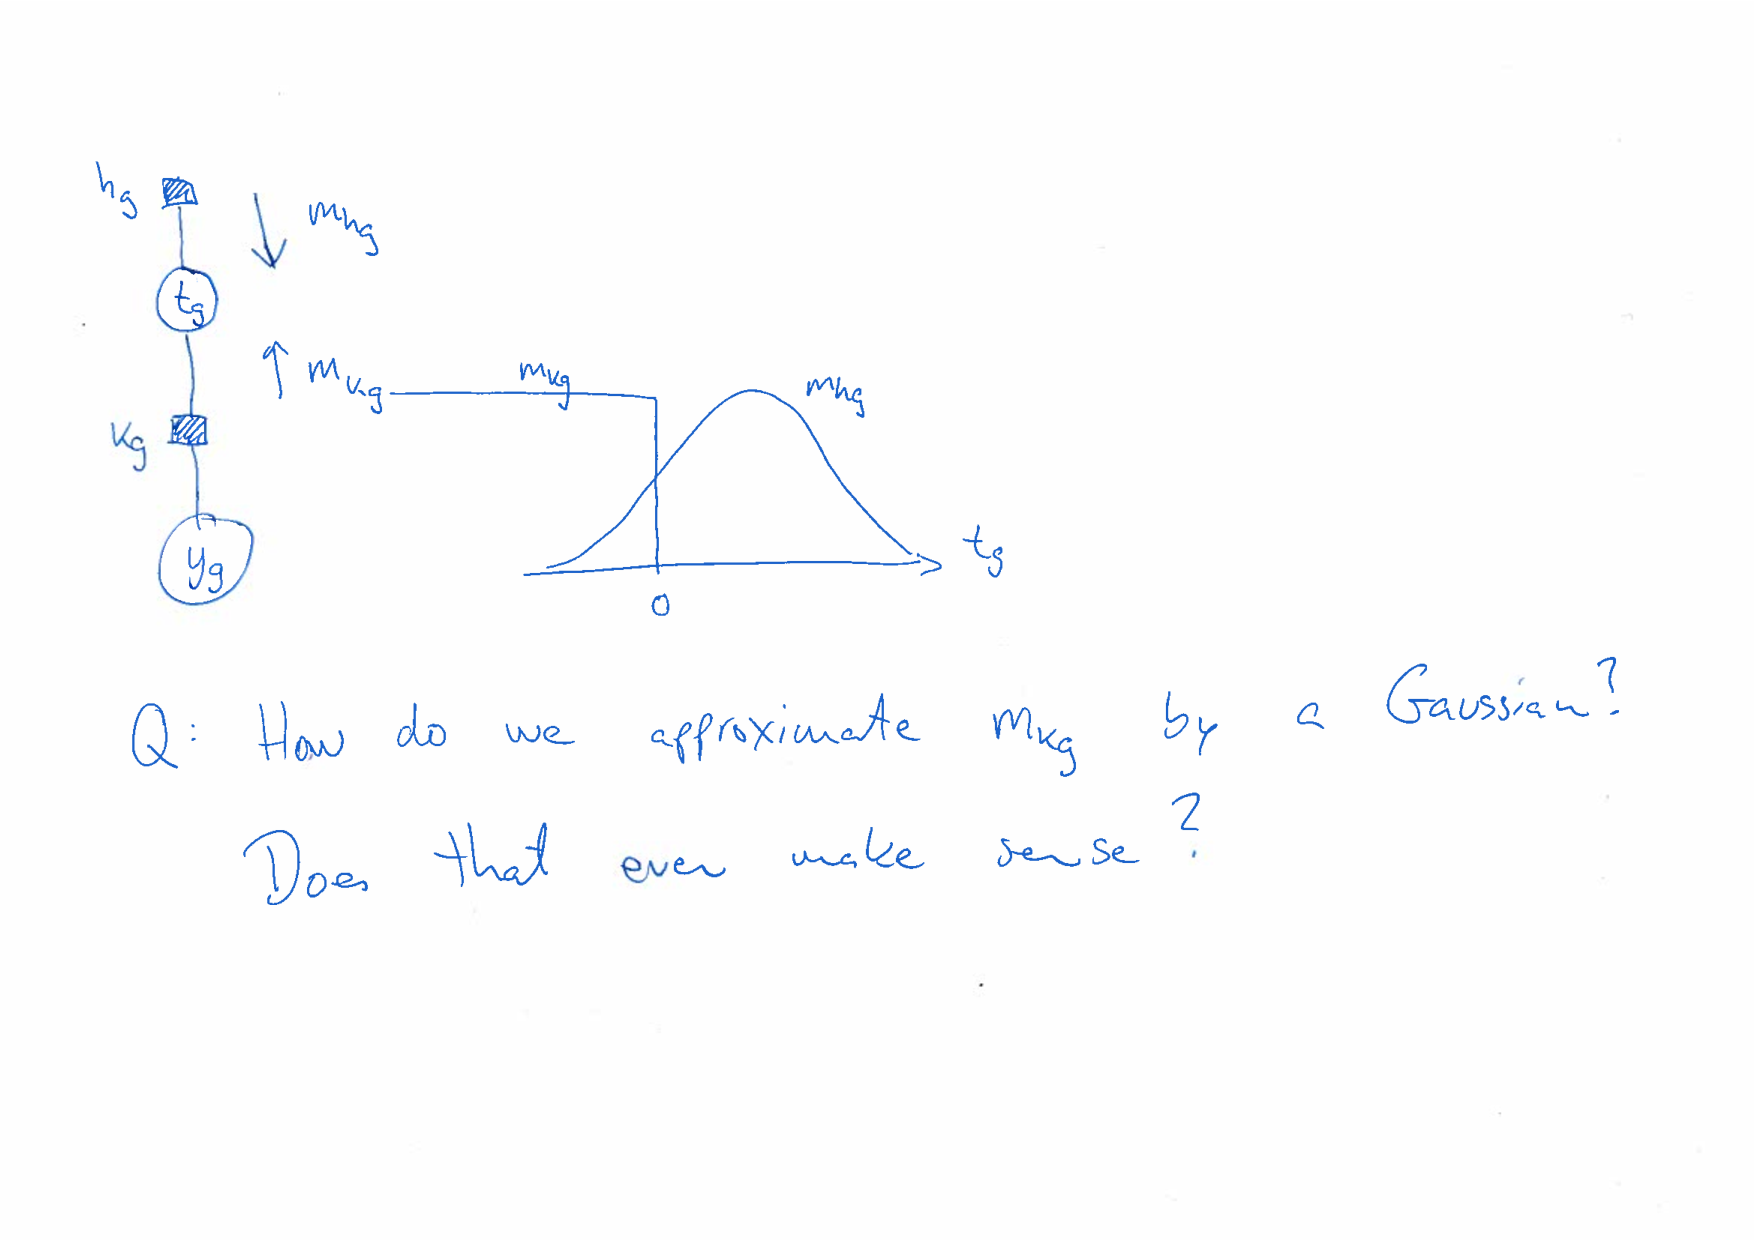
\includegraphics[width=\textwidth]{hand}}
\end{frame}


\begin{frame}
\frametitle{Moments of a truncated Gaussian density (1)}

Consider the truncated Gaussian density function
\[
p(t)\;=\;\frac{1}{Z_t}\delta\big(y-\operatorname{sign}(t)\big){\cal N}(t;\mu,\sigma^2)
\text{\ \ where\ \ }y\in\{-1, 1\}\text{\ \ and\ \ }\delta(x)=1\text{\ \ iff\ \ }x=0.
\]
\centerline{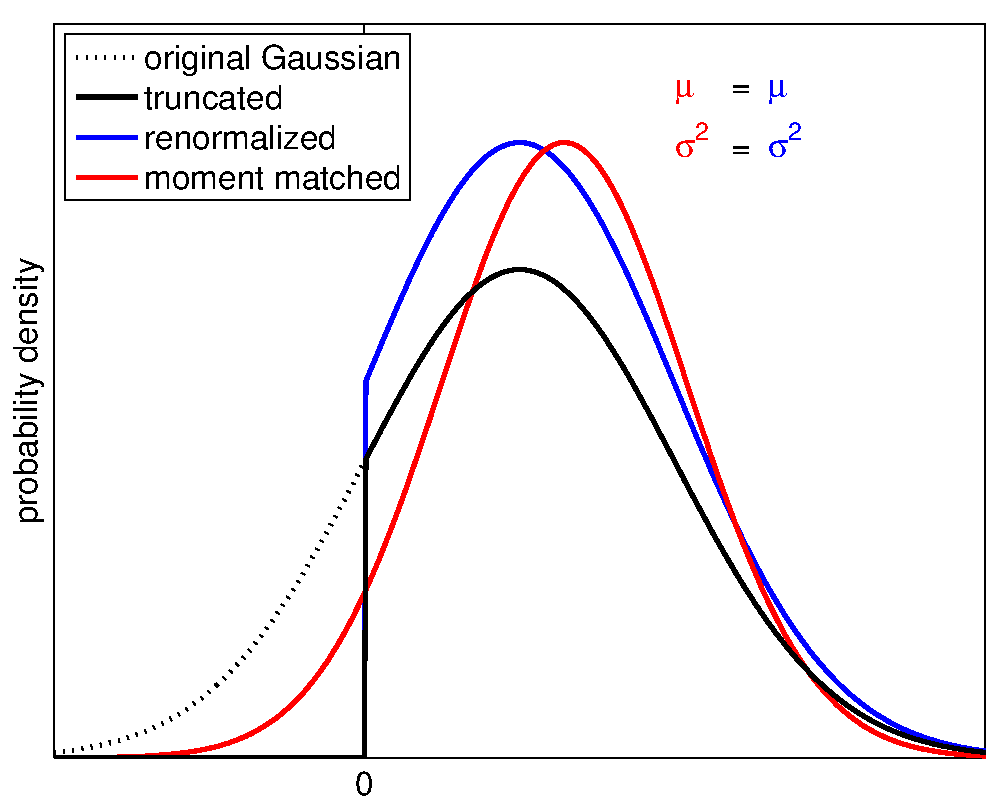
\includegraphics[width=0.4\textwidth]{momtruncgau}}

We want to \Blue{\emph{approximate}} $p(t)$ by a Gaussian density function $q(t)$
with mean and variance equal to the first and second central moments
of $p(t)$. We need:
\begin{itemize}
\item First moment: $\E[t] = \langle t\rangle_{p(t)}$
\item Second central moment: $\V[t] = \langle t^2\rangle_{p(t)} - \langle t \rangle^2_{p(t)}$
\end{itemize}

\end{frame}


\begin{frame}
\frametitle{Moments of a truncated Gaussian density (2)}

We have seen that the normalisation constant is $Z_t = \Phi\big(\frac{y\mu}{\sigma}\big)$. 

{\bf First moment}. We take the derivative of $Z_t$ wrt.\ $\mu$:
\begin{align*}
\frac{\partial Z_t}{\partial \mu} &= \frac{\partial}{\partial \mu} 
\int_0^{+\infty}\!\! N(t; y\mu, \sigma^2)\mathrm{d}t
= \int_0^{+\infty}\!  \frac{\partial}{\partial \mu}  N(t; y\mu, \sigma^2)\mathrm{d}t\\
&= \int_0^{+\infty}\! y\sigma^{-2}(t-y\mu) N(t; y\mu, \sigma^2)\mathrm{d}t
= y Z_t \sigma^{-2}\int_{-\infty}^{+\infty}\! (t-y\mu) p(t)\mathrm{d}t\\
&= y Z_t \sigma^{-2}\langle t-y\mu\rangle_{p(t)} 
= y Z_t \sigma^{-2}\langle t\rangle_{p(t)} - \mu Z_t \sigma^{-2}
\end{align*}
where $\langle t\rangle_{p(t)}$ is the expectation of $t$ under $p(t)$. We can also write:
\[
\frac{\partial Z_t}{\partial \mu} 
= \frac{\partial}{\partial \mu}\Phi\big(\frac{y\mu}{\sigma}\big)
= y \N(y\mu; 0, \sigma^2)
\]

Combining both expressions for $\frac{\partial Z_t}{\partial \mu}$
we obtain
\[
\langle t\rangle_{p(t)} = y\mu + \sigma^2\frac{\N(y\mu; 0, \sigma^2)}{\Phi(\frac{y\mu}{\sigma})}
= y\mu + \sigma\frac{\N(\frac{y\mu}{\sigma}; 0, 1)}{\Phi(\frac{y\mu}{\sigma})}
= y\mu + \sigma \Psi\big(\frac{y\mu}{\sigma}\big)
\]
where use $\N(y\mu; 0, \sigma^2) = \sigma^{-1}\N(\frac{y\mu}{\sigma}; 0, 1)$
and define $\Psi(z) = \frac{N(z; 0,1)}{\Phi(z)}$.

\end{frame}


\begin{frame}
\frametitle{Moments of a truncated Gaussian density (3)}

{\bf Second moment}. We take the second derivative of $Z_t$ wrt.\ $\mu$:
\begin{align*}
\frac{\partial^2 Z_t}{\partial \mu^2} &= \frac{\partial}{\partial \mu} 
\int_0^{+\infty}\! y\sigma^{-2}(t-y\mu) N(t; y\mu, \sigma^2)\mathrm{d}t\\
& = \Phi\big(\frac{y\mu}{\sigma}\big)\langle -\sigma^{-2} + \sigma^{-4}(t-y\mu)^2\rangle_{p(t)}
\end{align*}

We can also write
\[
\frac{\partial^2 Z_t}{\partial \mu^2} 
= \frac{\partial}{\partial \mu} y\N(y\mu; 0, \sigma^2)
= -\sigma^{-2} y \mu \N(y\mu; 0, \sigma^2)
\]

Combining both we obtain
\[
\V[t] = \sigma^2\big(1 - \Lambda(\frac{y\mu}{\sigma})\big)
\]
where we define $\Lambda(z) = \Psi(z)\big(\Psi(z) + z\big)$.

\end{frame}

\end{document}
